\section{Ablation Studies and Analysis}
\label{sec:exp:abl}

The previous section demonstrates that the learned controller tracks the diagnostic signals underlying the design of TurnOPD. We now turn to a more fine-grained question: How do individual budget controllers in TurnOPD contribute to its overall performance? 

To answer this, we conduct ablation studies on ALFWorld-1.7B (Qwen3-1.7B distilled from Qwen3-8B-GRPO on ALFWorld task) using the same 100-step protocol as in the main experiment. The analysis proceeds in three parts. First, we disentangle the two core interventions to evaluate whether each is effective on its own. Second, we ablate the KL normalization scheme, comparing trajectory-level, strict turn-level, and linear turn-level reductions. Third, we analyze the effect of altering the coverage floor, which determines the conservativeness of the adaptive-depth controller.

\subsection{Intervention Component Decomposition}
\label{sec:exp:intervention-decomposition}

This subsection analyzes the individual contribution of each TurnOPD budget controller to overall performance.

\textbf{Setup.}
We conduct experiments on the ALFWorld task.
The \textit{Adaptive Depth} variant applies the adaptive rollout-depth budget controller while keeping the original trajectory-level KL reduction unchanged, to test if simply shortening rollout depth is sufficient. In contrast, the \textit{Linear blend norm} variant maintains the full-horizon OPD rollout depth but replaces the KL reduction with a linear turn-level normalizer, assessing whether rebalancing loss allocation alone can be effective. The full TurnOPD approach integrates both budget controllers. We report the overall Avg@4 accuracy under full training, averaging the last four evaluation checkpoints.

\begin{figure}[tbp]
    \centering
    \begin{minipage}[c]{0.45\textwidth}
        \centering
        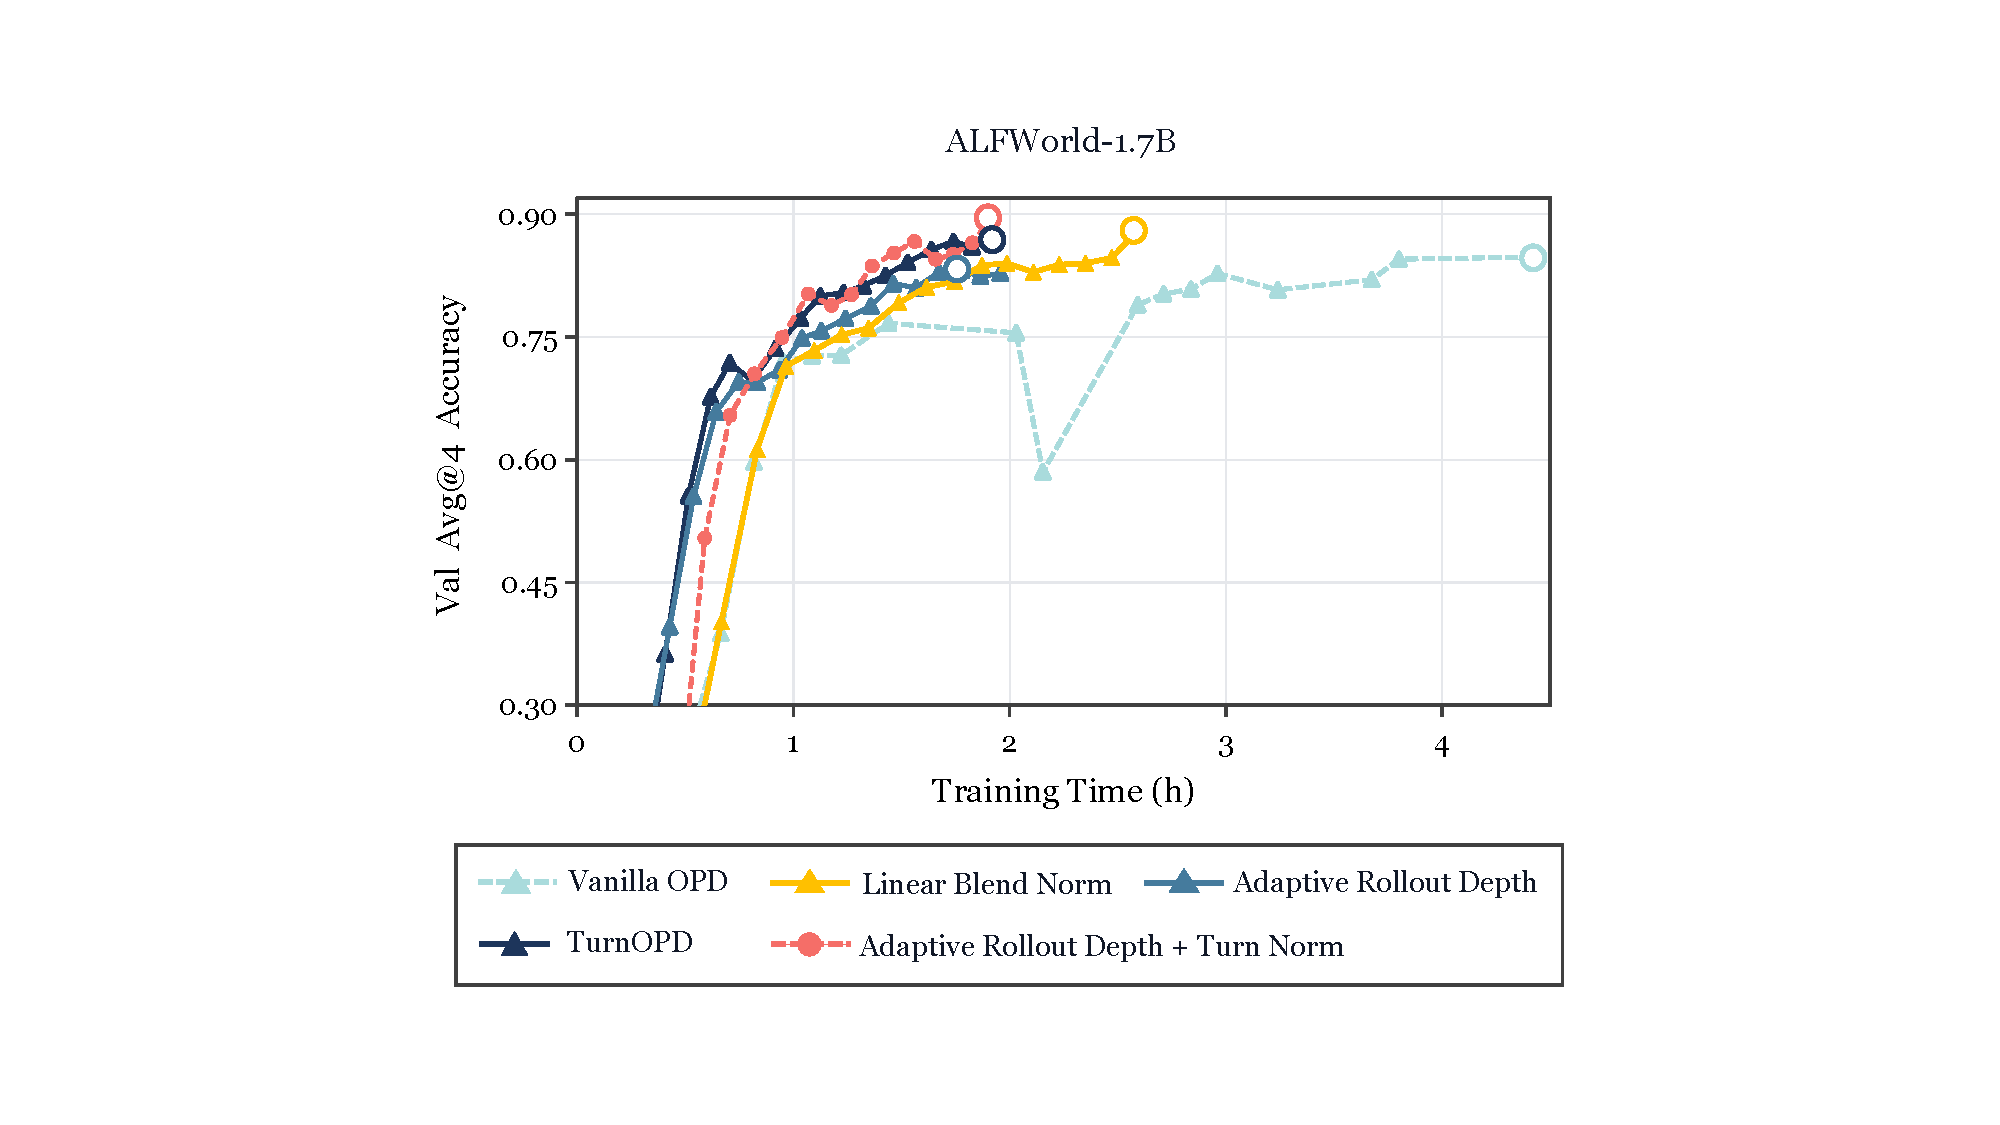
\includegraphics[width=\linewidth]{figures/component_ablation.pdf}
        \captionsetup{hypcap=false}
        \captionof{figure}{ALFWorld-1.7B component ablations.}
        \label{fig:ablation}
    \end{minipage}\hfill
    \begin{minipage}[c]{0.53\textwidth}
        \centering
        \captionsetup{hypcap=false}
        \captionof{table}{Intervention decomposition on ALFWorld-1.7B over the total
        100 optimizer steps. Acc reports Same-Step Avg@4, averaging the last four
        evaluation checkpoints. Wall time sums per-step training
        time over all training steps.}
        \label{tab:abl}
        \scriptsize
        \def\interventionTableWidth{0.98\linewidth}
        \setlength{\tabcolsep}{3pt}
        \renewcommand{\arraystretch}{0.96}
        \resizebox{\interventionTableWidth}{!}{%
        \begin{tabular}{@{}>{\raggedright\arraybackslash}m{2.2cm}>{\centering\arraybackslash}m{1cm}>{\centering\arraybackslash}m{1cm}>{\centering\arraybackslash}m{1.2cm}>{\centering\arraybackslash}m{1.2cm}@{}}
        \toprule
        Config & Depth & Blend & Avg@4 & Wall (h) \\
        \midrule
        Vanilla OPD          &        &        & 83.0 & 4.42 \\
        + Adaptive Depth          & \checkmark &     & 82.8 & 1.96 \\
        + Linear blend norm         &        & \checkmark & 85.1 & 2.59 \\
        \textbf{TurnOPD}        & \checkmark & \checkmark & \textbf{86.3} & \textbf{1.93} \\
        \bottomrule
        \end{tabular}}
    \end{minipage}
\end{figure}

\textbf{Results.}
Figure~\ref{fig:ablation} presents the full validation curves across training, while Table~\ref{tab:abl} summarizes the Same-Step Avg@4 accuracy and cumulative wall time after 100 optimizer steps.
The results support the intended division of labor. Adaptive depth alone cuts
the 100-step wall time from $4.42$ h to $1.96$ h, but its accuracy drops slightly from
$83.0$ to $82.8$. This indicates that reducing rollout depth is not a complete
training solution by itself: it saves compute, but it does not fix the loss
allocation problem identified in Section~\ref{sec:diag:turnnorm}. In contrast,
the linear KL blend improves accuracy to $85.1$, showing that the loss
allocator directly improves optimization, but it still costs $2.59$ h. 
Full TurnOPD combines the two effects: it achieves the best average accuracy ($86.3$) while matching the low wall time of the adaptive-depth run ($1.93$ h). Notably, using adaptive rollout depth together with turn-level KL normalization alone can sometimes yield final performance close to, or slightly higher than, TurnOPD. However, TurnOPD outperforms these alternatives in the middle stages of training, demonstrating faster progress and better intermediate results. Thus, the ablations tell a coherent story: the rollout-depth budget controller provides the efficiency lever, the progressive loss-budget controller provides the optimization lever, and their combination gives the best accuracy--time tradeoff.

\subsection{Effect of KL Normalization}
\label{sec:exp:kl-normalization}

\textbf{Motivation and Experiment Setup.}
Section~\ref{sec:diag:turnnorm} points out that KL loss normalization has a budget allocation problem: the standard (trajectory-level) approach mostly focuses on shallow turns, while a hard turn-level strategy can overcompensate and put too much weight on rarely supported deep turns. To better understand this, we compare three KL normalization schemes: \textbf{trajectory-level KL}, \textbf{hard turn-level KL}, and our \textbf{linear blend method}. For fairness, we report each method's Same-Step Avg@4 and the actual loss budget spent on the deepest third of valid turns (i.e., turns reached by enough trajectories).

\textbf{Results.}
As shown in Table~\ref{tab:abl-turnnorm}, trajectory-level KL is stable but strongly favors shallow turns: the deepest third gets only 3.2/0.7/1.2\% of the budget in early/mid/late training. Hard turn-level KL sharply reverses this, instantly giving around a third of the budget to deep turns, but makes an abrupt shift and may overweight unreliable estimates early on. Our linear blend offers a smoother transition: $\alpha$ rises from $0.17$ to $0.83$ across the early/mid/late phases, while the deep-turn budget increases from $12.8\%$ to $27.7\%$. This method balances stability and targeted allocation, yielding the best Same-Step Avg@4, though the margin over hard turn-level KL is small.

\begin{table*}[htbp]
\centering
\caption{
Impact of KL normalization strategies on ALFWorld-1.7B. ``Same-Step Avg@4'' is the mean over the last four evaluation checkpoints. ``Deep budget'' gives the KL budget assigned to the deepest third of valid turns in early/mid/late training. ``$\alpha$'' is the blend coefficient, with $\alpha=0$ for trajectory-level KL and $\alpha=1$ for hard turn-level KL.
}
\label{tab:abl-turnnorm}
\small
\setlength{\tabcolsep}{4pt}
\resizebox{0.85\textwidth}{!}{%
\begin{tabular}{
    @{}>{\raggedright\arraybackslash}m{4.5cm}>{\centering\arraybackslash}m{2.2cm}>{\centering\arraybackslash}m{3.2cm}>{\centering\arraybackslash}m{2.2cm}@{}}
\toprule
KL normalizer & \shortstack{Same-Step\\Avg@4} & \shortstack{Deep budget\\E/M/L} & \shortstack{$\alpha$\\E/M/L} \\
\midrule
Trajectory-level KL          & 83.0 & 3.2/0.7/1.2\% & 0/0/0 \\
Turn-level KL (hard switch)  & 85.0 & 29.9/32.0/31.9\% & 1/1/1 \\
\textbf{Linear blend (ours)} & \textbf{85.1} & 12.8/21.6/27.7\% & 0.17/0.50/0.83 \\
\bottomrule
\end{tabular}
}
\end{table*}

\subsection{Adaptive-Depth Coverage Sensitivity}
\label{sec:exp:coverage-sensitivity}

The Adaptive Rollout Depth module exposes two main hyperparameters: (1) the coverage quantile $p$, and (2) the choice of whether the completion cumulative distribution function (CDF) is computed from only successful trajectories or from the full trajectory population. In practice, many open-ended agentic tasks do not provide a reliable distinction between successful and unsuccessful trajectories. Moreover, the OPD algorithm itself does not fundamentally depend on a reward signal denoting task success. To assess robustness in more general settings, we conducted additional experiments evaluating the adaptive-depth controller without access to a success-conditioned CDF.

For this hyperparameter study, we swept $p\in\{0.4, 0.6, 0.8\}$ across both success-conditioned and full-population CDFs. Figure~\ref{fig:coverage-ablation} summarizes four diagnostic metrics: validation accuracy and EMA-smoothed rollout horizon (ema-H) for both the success-conditioned and full-population CDF settings. Here, ema-H refers to the exponentially smoothed average rollout depth, which directly determines the effective student rollout horizon. We summarize the main observations as follows:

\begin{figure}[htbp]
\centering
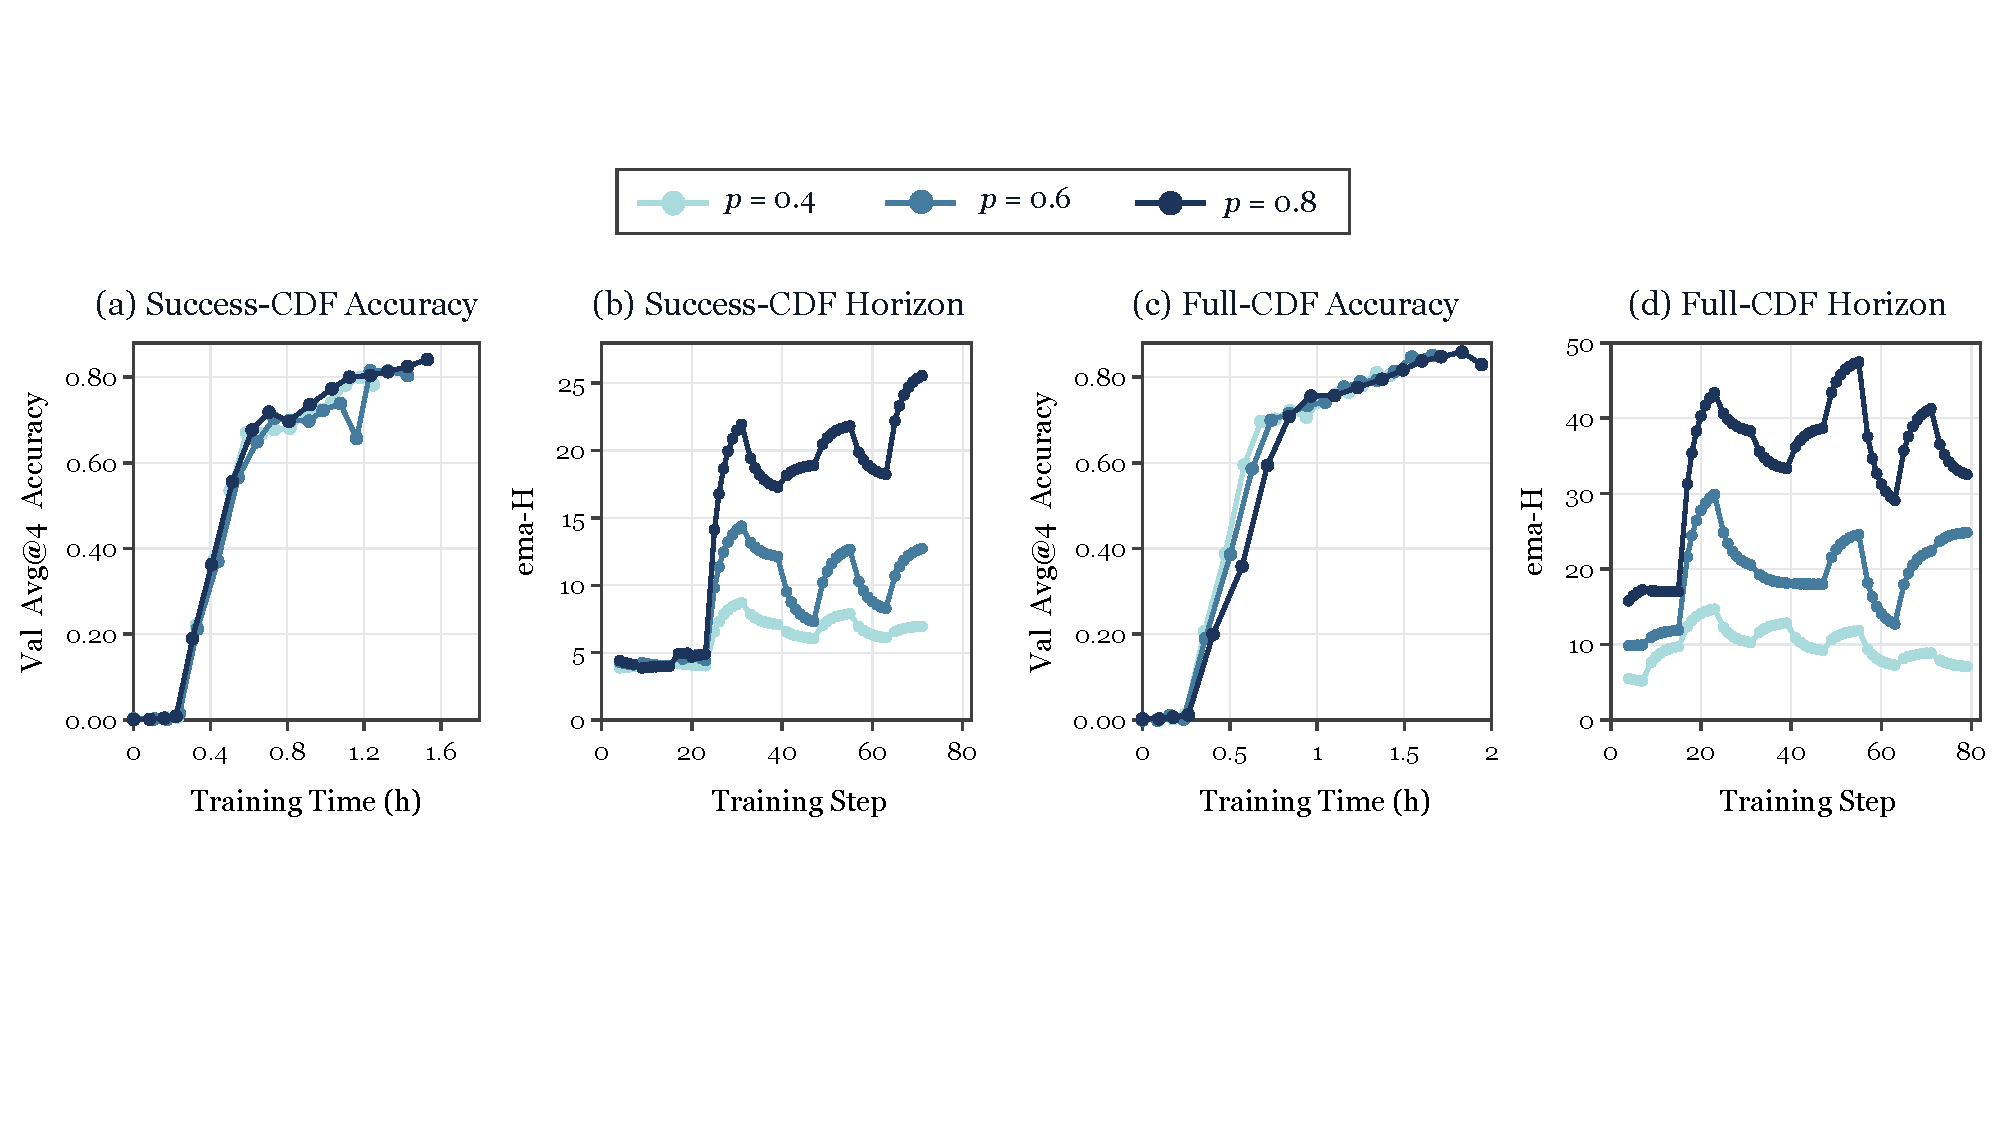
\includegraphics[width=\linewidth]{figures/CDF.pdf}
\caption{Coverage-floor sensitivity on ALFWorld-1.7B. The four panels show validation accuracy versus
cumulative training time and logged EMA horizon for the success-conditioned CDF
and the full-population CDF.}
\label{fig:coverage-ablation}
\end{figure}


\textbf{(1) The quantile parameter $p$ directly controls the target rollout horizon.} Increasing $p$ yields slightly higher final success rates, but also results in deeper rollout horizons and correspondingly increased training time. For example, with the full-population CDF, setting $p=0.6$ achieves an accuracy of 85.1 in 1.66 hours, while $p=0.8$ improves the accuracy to 85.8 but increases the required time to 1.83 hours.

\textbf{(2) The CDF source significantly affects efficiency.} The full-population CDF is more aggressive: it consistently increases ema-H and wall time compared to the success-conditioned CDF. This matches intuition, as the full-population CDF incorporates many failed trajectories, including those that stall at the maximum rollout depth due to repeated or unproductive tool usage, thereby overestimating the required depth. Nonetheless, as shown in the figure, the full-population CDF remains effective, but requires appropriately lower values of $p$ to match the efficiency and performance of the success-conditioned CDF.
